\documentclass[11pt,a4paper,]{article}
\usepackage{lmodern}

\usepackage{amssymb,amsmath}
\usepackage{ifxetex,ifluatex}
\usepackage{fixltx2e} % provides \textsubscript
\ifnum 0\ifxetex 1\fi\ifluatex 1\fi=0 % if pdftex
  \usepackage[T1]{fontenc}
  \usepackage[utf8]{inputenc}
\else % if luatex or xelatex
  \usepackage{unicode-math}
  \defaultfontfeatures{Ligatures=TeX,Scale=MatchLowercase}
\fi
% use upquote if available, for straight quotes in verbatim environments
\IfFileExists{upquote.sty}{\usepackage{upquote}}{}
% use microtype if available
\IfFileExists{microtype.sty}{%
\usepackage[]{microtype}
\UseMicrotypeSet[protrusion]{basicmath} % disable protrusion for tt fonts
}{}
\PassOptionsToPackage{hyphens}{url} % url is loaded by hyperref
\usepackage[unicode=true]{hyperref}
\hypersetup{
            pdftitle={Attention Towards Distance Education Tools During COVID-19 Pandemic: Evidence from Google Trends},
            pdfkeywords={rmarkdown, templates},
            pdfborder={0 0 0},
            breaklinks=true}
\urlstyle{same}  % don't use monospace font for urls
\usepackage{geometry}
\geometry{left=2.5cm,right=2.5cm,top=2.5cm,bottom=2.5cm}
\usepackage[style=authoryear-comp,]{biblatex}
\addbibresource{references.bib}
\usepackage{longtable,booktabs}
% Fix footnotes in tables (requires footnote package)
\IfFileExists{footnote.sty}{\usepackage{footnote}\makesavenoteenv{long table}}{}
\IfFileExists{parskip.sty}{%
\usepackage{parskip}
}{% else
\setlength{\parindent}{0pt}
\setlength{\parskip}{6pt plus 2pt minus 1pt}
}
\setlength{\emergencystretch}{3em}  % prevent overfull lines
\providecommand{\tightlist}{%
  \setlength{\itemsep}{0pt}\setlength{\parskip}{0pt}}
\setcounter{secnumdepth}{5}

% set default figure placement to htbp
\makeatletter
\def\fps@figure{htbp}
\makeatother


\title{Attention Towards Distance Education Tools During COVID-19 Pandemic: Evidence from Google Trends}

%% MONASH STUFF

%% CAPTIONS
\RequirePackage{caption}
\DeclareCaptionStyle{italic}[justification=centering]
 {labelfont={bf},textfont={it},labelsep=colon}
\captionsetup[figure]{style=italic,format=hang,singlelinecheck=true}
\captionsetup[table]{style=italic,format=hang,singlelinecheck=true}

%% FONT
\RequirePackage{bera}
\RequirePackage{mathpazo}

%% HEADERS AND FOOTERS
\RequirePackage{fancyhdr}
\pagestyle{fancy}
\rfoot{\Large\sffamily\raisebox{-0.1cm}{\textbf{\thepage}}}
\makeatletter
\lhead{\textsf{\expandafter{\@title}}}
\makeatother
\rhead{}
\cfoot{}
\setlength{\headheight}{15pt}
\renewcommand{\headrulewidth}{0.4pt}
\renewcommand{\footrulewidth}{0.4pt}
\fancypagestyle{plain}{%
\fancyhf{} % clear all header and footer fields
\fancyfoot[C]{\sffamily\thepage} % except the center
\renewcommand{\headrulewidth}{0pt}
\renewcommand{\footrulewidth}{0pt}}

%% MATHS
\RequirePackage{bm,amsmath}
\allowdisplaybreaks

%% GRAPHICS
\RequirePackage{graphicx}
\setcounter{topnumber}{2}
\setcounter{bottomnumber}{2}
\setcounter{totalnumber}{4}
\renewcommand{\topfraction}{0.85}
\renewcommand{\bottomfraction}{0.85}
\renewcommand{\textfraction}{0.15}
\renewcommand{\floatpagefraction}{0.8}

%\RequirePackage[section]{placeins}

%% SECTION TITLES
\RequirePackage[compact,sf,bf]{titlesec}
\titleformat{\section}[block]
  {\fontsize{15}{17}\bfseries\sffamily}
  {\thesection}
  {0.4em}{}
\titleformat{\subsection}[block]
  {\fontsize{12}{14}\bfseries\sffamily}
  {\thesubsection}
  {0.4em}{}
\titlespacing{\section}{0pt}{*5}{*1}
\titlespacing{\subsection}{0pt}{*2}{*0.2}


%% TITLE PAGE
\def\Date{\number\day}
\def\Month{\ifcase\month\or
 January\or February\or March\or April\or May\or June\or
 July\or August\or September\or October\or November\or December\fi}
\def\Year{\number\year}

\makeatletter
\def\wp#1{\gdef\@wp{#1}}\def\@wp{??/??}
\def\jel#1{\gdef\@jel{#1}}\def\@jel{??}
\def\showjel{{\large\textsf{\textbf{JEL classification:}}~\@jel}}
\def\nojel{\def\showjel{}}
\def\addresses#1{\gdef\@addresses{#1}}\def\@addresses{??}
\def\cover{{\sffamily\setcounter{page}{0}
        \thispagestyle{empty}
        \vspace*{2cm}
        \begin{center}
        \fbox{\parbox{14cm}{\begin{onehalfspace}\centering\Huge\vspace*{0.3cm}
                \textsf{\textbf{\expandafter{\@title}}}\vspace{1cm}\par
                \LARGE\@author\end{onehalfspace}
        }}
        \end{center}
        \vfill
                \begin{center}\Large
                \Month~\Year\\[1cm]
                Working Paper \@wp
        \end{center}\vspace*{2cm}}}
\def\pageone{{\sffamily\setstretch{1}%
        \thispagestyle{empty}%
        \vbox to \textheight{%
        \raggedright\baselineskip=1.2cm
     {\fontsize{24.88}{30}\sffamily\textbf{\expandafter{\@title}}}
        \vspace{2cm}\par
        \hspace{1cm}\parbox{14cm}{\sffamily\large\@addresses}\vspace{1cm}\vfill
        \hspace{1cm}{\large\Date~\Month~\Year}\\[1cm]
        \hspace{1cm}\showjel\vss}}}
\def\blindtitle{{\sffamily
     \thispagestyle{plain}\raggedright\baselineskip=1.2cm
     {\fontsize{24.88}{30}\sffamily\textbf{\expandafter{\@title}}}\vspace{1cm}\par
        }}
\def\titlepage{{\cover\newpage\pageone\newpage\blindtitle}}

\def\blind{\def\titlepage{{\blindtitle}}\let\maketitle\blindtitle}
\def\titlepageonly{\def\titlepage{{\pageone\end{document}}}}
\def\nocover{\def\titlepage{{\pageone\newpage\blindtitle}}\let\maketitle\titlepage}
\let\maketitle\titlepage
\makeatother

%% SPACING
\RequirePackage{setspace}
\spacing{1.5}

%% LINE AND PAGE BREAKING
\sloppy
\clubpenalty = 10000
\widowpenalty = 10000
\brokenpenalty = 10000
\RequirePackage{microtype}

%% PARAGRAPH BREAKS
\setlength{\parskip}{1.4ex}
\setlength{\parindent}{0em}

%% HYPERLINKS
\RequirePackage{xcolor} % Needed for links
\definecolor{darkblue}{rgb}{0,0,.6}
\RequirePackage{url}

\makeatletter
\@ifpackageloaded{hyperref}{}{\RequirePackage{hyperref}}
\makeatother
\hypersetup{
     citecolor=0 0 0,
     breaklinks=true,
     bookmarksopen=true,
     bookmarksnumbered=true,
     linkcolor=darkblue,
     urlcolor=blue,
     citecolor=darkblue,
     colorlinks=true}

%% KEYWORDS
\newenvironment{keywords}{\par\vspace{0.5cm}\noindent{\sffamily\textbf{Keywords:}}}{\vspace{0.25cm}\par\hrule\vspace{0.5cm}\par}

%% ABSTRACT
\renewenvironment{abstract}{\begin{minipage}{\textwidth}\parskip=1.4ex\noindent
\hrule\vspace{0.1cm}\par{\sffamily\textbf{\abstractname}}\newline}
  {\end{minipage}}


\usepackage[T1]{fontenc}
\usepackage[utf8]{inputenc}

\usepackage[showonlyrefs]{mathtools}
\usepackage[no-weekday]{eukdate}

%% BIBLIOGRAPHY

\makeatletter
\@ifpackageloaded{biblatex}{}{\usepackage[style=authoryear-comp, backend=biber, natbib=true]{biblatex}}
\makeatother
\ExecuteBibliographyOptions{bibencoding=utf8,minnames=1,maxnames=3, maxbibnames=99,dashed=false,terseinits=true,giveninits=true,uniquename=false,uniquelist=false,doi=false, isbn=false,url=true,sortcites=false}

\DeclareFieldFormat{url}{\texttt{\url{#1}}}
\DeclareFieldFormat[article]{pages}{#1}
\DeclareFieldFormat[inproceedings]{pages}{\lowercase{pp.}#1}
\DeclareFieldFormat[incollection]{pages}{\lowercase{pp.}#1}
\DeclareFieldFormat[article]{volume}{\mkbibbold{#1}}
\DeclareFieldFormat[article]{number}{\mkbibparens{#1}}
\DeclareFieldFormat[article]{title}{\MakeCapital{#1}}
\DeclareFieldFormat[inproceedings]{title}{#1}
\DeclareFieldFormat{shorthandwidth}{#1}
% No dot before number of articles
\usepackage{xpatch}
\xpatchbibmacro{volume+number+eid}{\setunit*{\adddot}}{}{}{}
% Remove In: for an article.
\renewbibmacro{in:}{%
  \ifentrytype{article}{}{%
  \printtext{\bibstring{in}\intitlepunct}}}

\makeatletter
\DeclareDelimFormat[cbx@textcite]{nameyeardelim}{\addspace}
\makeatother
\renewcommand*{\finalnamedelim}{%
  %\ifnumgreater{\value{liststop}}{2}{\finalandcomma}{}% there really should be no funny Oxford comma business here
  \addspace\&\space}


\wp{1}
\jel{C10,C14,C22}

\RequirePackage[absolute,overlay]{textpos}
\setlength{\TPHorizModule}{1cm}
\setlength{\TPVertModule}{1cm}
\def\placefig#1#2#3#4{\begin{textblock}{.1}(#1,#2)\rlap{\includegraphics[#3]{#4}}\end{textblock}}




\author{Priyanga Dilini~Talagala, Thiyanga~Talagala}
\addresses{\textbf{Priyanga Dilini Talagala}\newline
Department of Compuational Mathematics, University of Moratuwa, Sri Lanka
\newline{Email: \href{mailto:priyangad@uom.lk}{\nolinkurl{priyangad@uom.lk}}}\newline Corresponding author\\[1cm]
\textbf{Thiyanga Talagala}\newline
Department of Statistics, University of Sri Jayewardenepura, Sri Lanka
\newline{Email: \href{mailto:tstalagala@gmail.com}{\nolinkurl{tstalagala@gmail.com}}}\\[1cm]
}

\date{\sf\Date~\Month~\Year}
\makeatletter
 \lfoot{\sf Talagala, Talagala: \@date}
\makeatother

%% Any special functions or other packages can be loaded here.


\begin{document}
\maketitle
\begin{abstract}
A brief summary of our work
\end{abstract}
\begin{keywords}
rmarkdown, templates
\end{keywords}

\hypertarget{introduction}{%
\section{Introduction}\label{introduction}}

The ongoing pandemic of COVID-19 has now become the most important priority of governments and media of many countries all around the world. Due to the alarming levels of spread and severity, the World Health Organization (WHO) declared the outbreak a Public Health Emergency of International (PHEIC) Concern on 30 January 2020, and then a pandemic on 11 March 2020 \autocite{world2020timeline}. As of 29 September 2021, more than 232.7 million cases of COVID-19 have been reported in over 192 countries and territories, resulting in more than 4.7 million deaths \autocite{dong2020interactive}. In response to the pandemic, health authorities worldwide have taken many steps including vaccination development and deployment to minimize the spread of the virus. In addition, authorities worldwide have also taken many non-pharmaceutical interventions and preventive measures such as travel restrictions, lock-downs, workplace hazard controls, school/university closures, facility closures, reduction of mass gatherings to reduce the spread of the virus \autocite{chang2020modelling}.

The first confirmed case of Covid-19 was reported from Sri Lanka on 27 January 2020 with a Chinese national who came to Sri Lanka as a tourist. The first locally transmitted COVID-19 case in Sri Lanka was then reported on 11 March 2020 followed by an increasing trend of the COVID-19 confirmed cases. In response to this increasing trend of COVID 19 cases, lockdowns and curfews were imposed several times across the country with the aim of reducing the spread of the virus. As of 29 September 2021, 515524 cases of COVID-19 have been reported in Sri Lanka, resulting with 12786 deaths \autocite{HealthSL2020,dong2020interactive}.

\begin{figure}[h]

{\centering 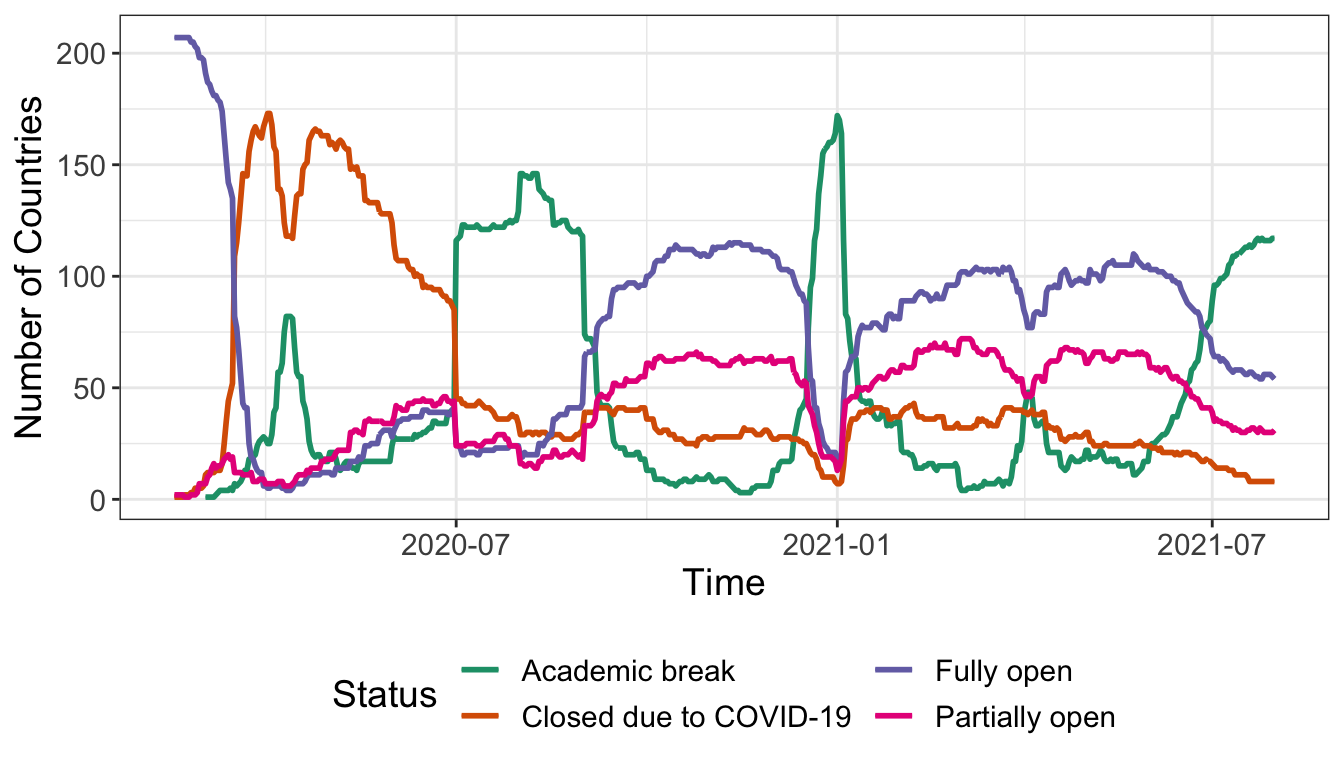
\includegraphics[width=1\textwidth]{figure/covidImpactWorld-1} 

}

\caption{Global tracking of COVID-19 caused school closures and re-openings}\label{fig:covidImpactWorld}
\end{figure}

\begin{figure}[h]

{\centering 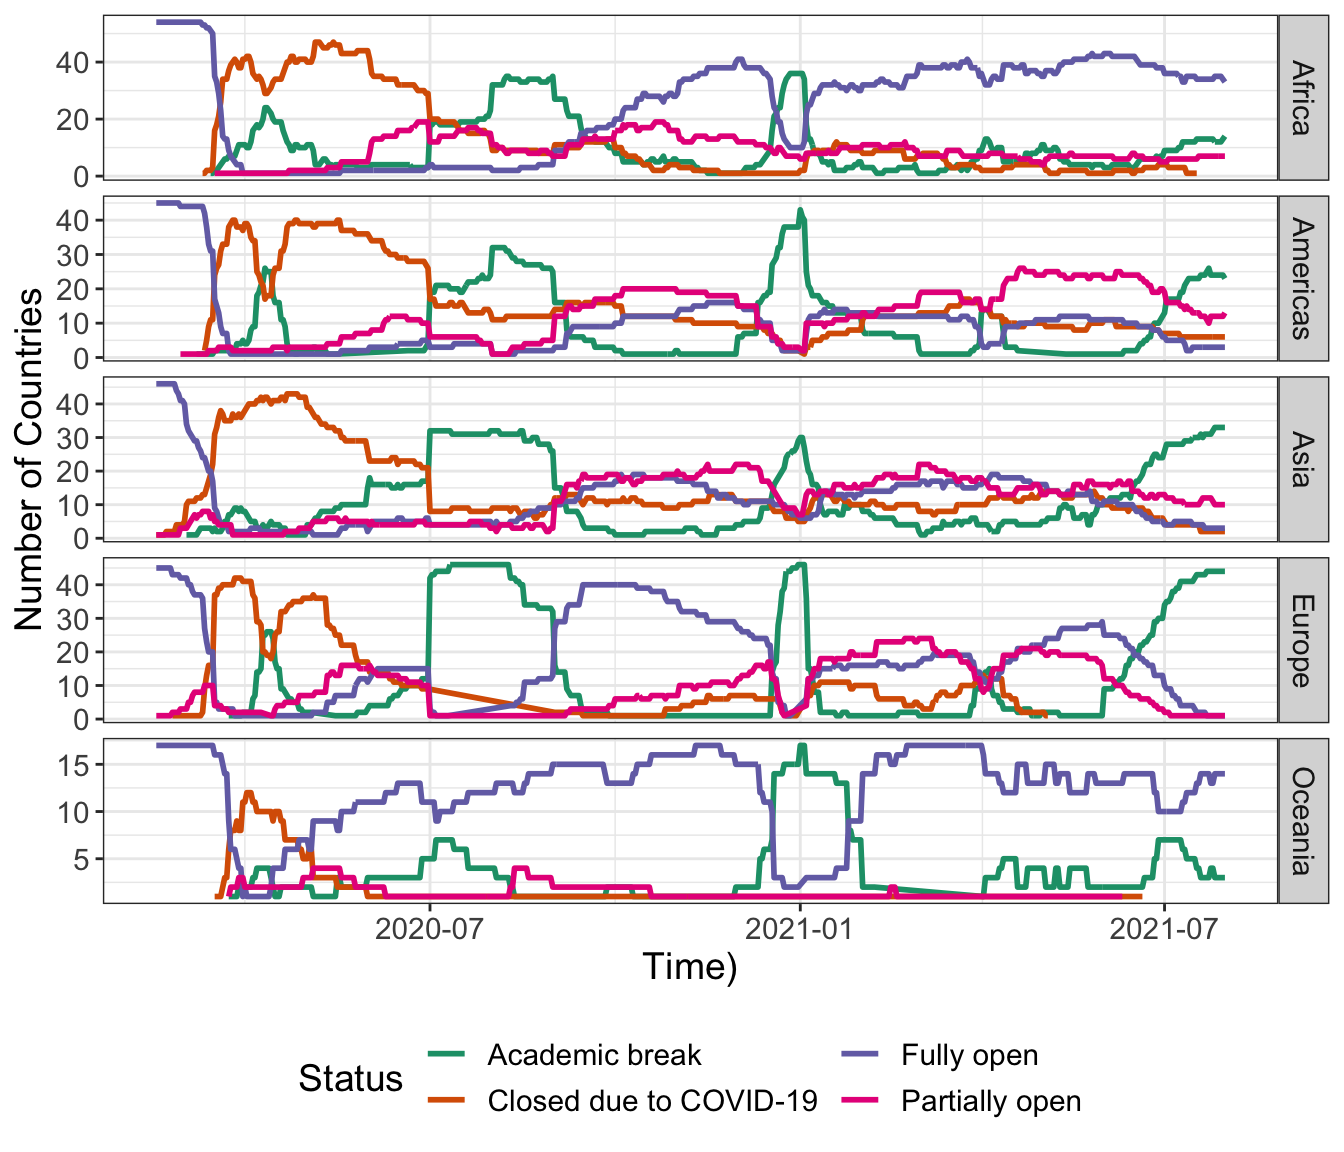
\includegraphics[width=1\textwidth]{figure/covidImpactContinent-1} 

}

\caption{Region wise tracking of COVID-19 caused school closures and re-openings}\label{fig:covidImpactContinent}
\end{figure}

The ongoing COVID-19 pandemic has brought the world to a standstill. Many sectors have been affected ever since the outbreak of COVID 19, worldwide. Among these many sectors education is one of the most affected sectors with a near-total closures of schools, colleges and universities, all around the world \autocite{daniel2020education}. Figures \ref{fig:covidImpactWorld} shows the evolution of global school closures and reopening since mid February 2020. With the start of the pandemic a near total closure of schools were observed all around the world. In line with that, the Sri Lankan government also ordered to close schools from 12 March 2020 and its planned reopening of schools was delayed several times due to unexpected Covid-19-related circumstances \autocite{wikieducation}. Over time, Africa and Oceania demonstrated better recovery in comparison to other regions with their increasing number of fully open schools (Figures \ref{fig:covidImpactWorld}).

Eventhough distance education has a long history that goes back to almost two centuries \autocite{spector2014handbook} with significant modifications,
alterations, and addition in the process of delivery and communication \autocite{moore2011learning}, COVID 19 certainly made a new era of distance education while encouraging various stakeholders of education to take the concept of distance education seriously. Sudden unexpected movement from classrooms to home schooling at large scale made students, teachers and parents vulnerable, leading to millions of education related internet searches being performed during the period of COVID 19 pandemic (Figures \ref{fig:distanceLearningWorldAnalysis}). Surprisingly, the search spikes of distance education related searches coincide with increasing Covid-19 counts and related internet searches, eventhough distance education has a long history in contrast to Covid-19 pandemic.

\begin{figure}[h]

{\centering 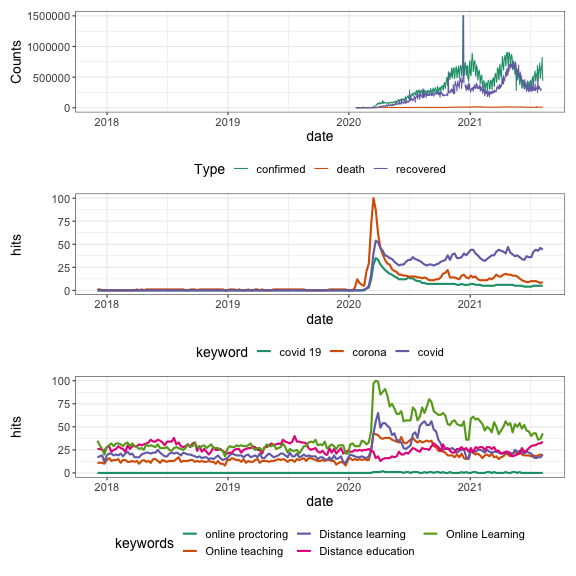
\includegraphics[width=1\textwidth]{figure/distanceLearningWorldAnalysis-1} 

}

\caption{Google trends footprint analysis}\label{fig:distanceLearningWorldAnalysis}
\end{figure}

The speed of these closures and the rapid move to online delivery of education allowed little time for planning or reflection on potential risks that could happen to its various stakeholders. The parents with limited education and resources; and students who tend to have fewer educational opportunities beyond schools and universities severely affected from this sudden unexpected movement. Further, the impact was not limited to students' learning but also to other aspects of their lives such as student debt, digital exclusion, lack of technology, lack of access to internet-enabled device or a stable internet connection, long-term educational disengagement, poor nutrition and food insecurity, increased psychological challenges, childcare problems, exploitation, school dropouts and lack of disability services. Teachers on the other hand were not fully aware of their obligations and how to maintain connections with students to support thier learning. Lack of preparation, lack of tools and techniques for distance education, lack of awareness of the availability of the existing tools and techniques and their effectiveness, lack of interaction and communication with the students, lack of awareness of students' ongoing problems were some of the major issues they encountered during COVID 19 pandemic \autocite{drane2020impact,daniel2020education,unescoadverse2020}. How to preparing course materials, How to interact with students, how to assess and evaluate student work, how to provide feedback are some major concerns they had when preparing for their first online teaching experience. Limited time, and lack of knowledge about the best online tools and techniques available were some of the major challenges teachers encountered during the online course preparation. This also put an extra burden on parents, specially with limited education and resources, as they were expected to facilitate the required learning environment at home.

In response to this grey situation and urgent requirement of massive transformation from physical classroom to virtual learning environment, UNESCO took immediate and timely action by publishing a list of distance learning solutions that can be used to facilitate student learning during the period of school closure. there are many different distance learning solutions. The design of different types of distance learning solutions can depend on the learning objective, target audience, access, and type of content \autocite{moore2011learning}. However, getting familiar with all these available distance solutions is not feasible or practical due to limited time availability and need of urgent responses.

The popularity of a product greatly influences consumer purchasing decisions can indicate its prominence in the market, its usability and its impact \autocite{ahn2006utilizing}. Further, according to \textcite{willis2020using}, developers also tend to improve the their products and services in response to increasing online search. Therefore, the Internet represents a great opportunity to learn about public attention towards a product or service. It's also a way to narrow down thier search space and thereby identify suitable tools and techniques to create an appropriate learning environment.

Google Trends is an open source web analytics tool that allows users to interact with Internet search data, which can provide deep insights into population behavior \autocite{nuti2014use}. In this paper we test whether the Google Analytics search index series can be used as a proxy of the popularity and the public interest in distance education solutions. In line with that, this paper makes three fundamental contributions to distance education by exploring three main questions: (1) What is the impact of COVID 19 pandemic on education? (2) What solutions are in place to meet the need of distance education in terms of coverage, up-take, and learning during COVID 19 pandemic? (3) Which solutions have a wide attention and public interest both at the national and global level?
We primarily analyze quantitative digital footprint data on the Internet from December 2019 to August 2021.The google trend footprint will allow the teachers to narrow down thier search space and select prominent distance education solutions for their teaching purposes.

The remainder of this paper is organized as follows. Section 2 presents the related work to lay the foundation for the Google footprint analysis. Section 3 presents the methodology followed in the study. Section 4 includes Google footprint analysis. Section 5 concludes the article and presents future research directions.

\hypertarget{background}{%
\subsection{Background}\label{background}}

\hypertarget{benefits-of-competition}{%
\subsubsection{Benefits of Competition}\label{benefits-of-competition}}

As Uber was queried more on Google, he was able to find a decrease in complaints of broken credit card machines as the taxis improved their service in response to the increased. Complaints may provide a proxy of the quality of traditional taxis in the city and thus provide a means to investigate the service quality differences in yellow taxis since the arrival of Uber \autocite{willis2020using}.

In total, our approach to employ novel data from a news media outlet to approximate the public interest and Uber's popularity enabled us to illustrate how Uber disrupted the New York City well established taxi market.

Both of these behavioural mechanisms can potentially explain the increase in the number of complaints about taxi service.
\#\# Analysis

\url{https://www.weforum.org/agenda/2020/12/google-most-popular-search-2020/}

Google has analyzed the billions of search requests it processes every day, and identified the terms that have had the highest spike this year compared to 2019. Unsurprisingly, ``coronavirus'' topped the overall list.

The search trends show the impact of the COVID pandemic on so many aspects of life. Relatively obscure teleconferencing company Zoom became a household name (and highly profitable business) as employees adapted to working from home, and friends and families turned to video calls instead of meeting in person .

Google Classroom was one of several online resources that provided education to millions of children affected by school closures. Searches for ``how to foster a dog'' reached an all-time high as social distancing triggered a yearning for the companionship of a pet.

\url{https://www.weforum.org/agenda/2020/12/google-most-popular-search-2020/}

Notably, GT, together with social media, could be use- fully exploited by global and local health agencies, as well as by public health practitioners, as a tool to identify disease-related information needs, social and behavioural barriers to infection control, and misinformation, as well as to better understand sentiment and risk perception as- sociated with health-threatening events such as an Ebola outbreak {[}5, 37{]}. Indeed, analyses of the temporal trend of GT-based query volumes together with their geographic distribution and main topics of searches can furnish a quantifiable and valuable measure of public attention and information needs about a particular communicable disease \autocite{alicino2015assessing}.

The Internet represents a great opportunity for public health agencies to disseminate healthcare-related infor- mation quickly, effectively and cheaply, provided that re- liable news are shared with as much of the population as possible, both in developed and developing countries, where the diffusion of new technologies among the population is rapidly increasing. Google Trends -- a pub- licly available data source -- could be used as a proxy of the proper diffusion of strategies based on health educa- tion messages, allowing to fill the translation gap be- tween best evidence (what some experts know) and practice (what most people do or believe) {[}38{]}. More- over, it could be exploited to determine the level of up- take of information about a public health event. Even during the 2014 Ebola outbreak, some stakeholders lev- eraged new technologies to plan proper communication strategies and address public concern {[}39, 40 \autocite{alicino2015assessing}.

Hara and Kling (2000) argue that more research about online courses from the students' perspective is needed. In a case study of graduate students enrolled in an online course, they found that many aspects of the course frustrated students, and that the instructor remained unaware of the continuing level of frustration. They suggest that many researchers bring an optimistic, romantic view of technology that may dampen their ability to look at hard questions and apply rigorous research methods. Much of the research, they maintain, has been advocacy and theorizing about future possibilities \autocite{wallace2003online}.

As shown in this literature review, the most common applications of Google search data in social science to date have been in economics, finance, and business, though there have also been studies in other fields, including media and technology (Rech, 2007), the entertainment industry (Goel, Hofman, Lahaie, Pennock, \& Watts, 2010), and politics (Reilly, Richey, \& Taylor, 2012). We did not, however, find any studies using Google Trends data in the higher education sector, which is our area of study \autocite{vaughan2014web}. However their (\textcite{vaughan2014web}) fous is on Our study determines whether Google Trends data can be used to estimate or predict academic fame by testing the correlation between search volume data and university ranking data.

\hypertarget{analysis}{%
\subsection{Analysis}\label{analysis}}

Every single step including planning, developing new tools and techniques, conducting awareness programs and workshops about online education, shifting towards online education happens through online due to unexpected massive shutdown worldwide.

\printbibliography

\end{document}
